Durante il periodo di Analisi tutta la documentazione da presentare in ingresso in sede di 
Revisione dei Requisiti è stata sottoposta ad una meticolosa attività di verifica. 
In questa sezione vengono descritti e analizzati gli esiti delle attività di verifica svolte su tutti i documenti che 
vengono consegnati nelle varie revisioni di avanzamento del progetto.

\subsection{Revisione}
\subsubsection{Revisione dei Requisiti}
\paragraph{Analisi statica dei documenti}\mbox{}\\
L'analisi dei documenti mediante \textit{Walkthrough}\glo{} ha portato 
all'individuazione di alcuni errori frequenti a partire dai quali è stata 
stilata una lista di controllo interna. In questo modo sarà possibile applicare
l'\textit{Inspection}\glo{} per le future attività di verifica.

L’analisi dei documenti mediante \textit{Walkthrough}\glo{} ha portato all’individuazione di alcuni errori frequenti. 
Una volta redatto il documento, il \textit{Verificatore} ne ha valutato poi la correttezza, nella sua interezza, cercando di individuarvi eventuali errori presenti. 
Se trovati la metodologia adottata è stata la seguente:
\begin{itemize}
    \item correzione degli errori ortografici e sintattici non conformi alle norme tipografiche stabilite nelle \textit{Norme di progetto v1.0.0};
    \item inserimento degli errori più ricorrenti nella \textit{lista di controllo}\glo{}, redatta durante la fase di verifica dei documenti;
    \item applicazione del ciclo \textit{PDCA}\glo{}, per migliorare e velocizzare le verifiche future. 
\end{itemize} 

A questo punto si è impiegata la tecnica dell'\textit{Inspection}\glo{}. 
Grazie alla \textit{lista di controllo}\glo{} si è infatti potuto svolgere un ulteriore esame nei confronti del documento sottoposto a verifica, per scoprire quegli errori che seppur presenti, non fossero stati ancora individuati dalle attività precedenti.


\subsubsection{Esito Revisione dei Requisiti}
Successivamente alla prima revisione, il gruppo, basandosi sulle segnalazioni ricevute, 
ha apportato varie modifiche ai documenti. Di seguito vengono descritte brevemente tali modifiche:
\begin{itemize}
    \item \textbf{Norme di progetto:} è stata aggiunta una sezione riguardante la formazione dei membri del gruppo e aggiornati gli strumenti di comunicazione esterni;
    \item \textbf{Analisi dei Requisiti:} seguendo le indicazioni del professor Cardin sono state apportate modifiche ai casi d'uso e ai requisiti, inoltre sono stati aggiunti i requisiti non funzionali;
    \item \textbf{Piano di Progetto:} è stato aggiunto il consuntivo di periodo tra la revisione dei requisiti e la revisione di progetto. Sono state fatte delle modifiche riguardanti il modello incrementale suggerite dal proponente Vardanega. Inoltre, è stato spostato in appendice il riscontro dei rischi;
    \item \textbf{Piano di Qualifica:} sono stati aggiornati i test di accettazione rispetto all’aggiornamento dei requisiti funzionali;
    \item \textbf{Glossario:} è stato modificata l'indicizzazione del glossario affinchè il suo utilizzo sia più corretto.
\end{itemize} 




\subsubsection{Revisione di progettazione}
\paragraph{Analisi statica del codice}\mbox{}\\
La stesura del codice è supportata dai plugin dell'editor Visual Studio Code. I plugin rilevanti in ambito di verifica sono due:
\begin{itemize}
    \item \textbf{\glo{ESlint} v2.1.10:}  linter per il linguaggio Javascript;
    \item \textbf{\glo{SonarLint} v1.20.0}  linter per diversi linguaggi di programmazione.
\end{itemize} 

I linter hanno aiutato notevolmente la stesura di codice sintatticamente corretto e alla standardizzazione del codice scritto, che risulta più uniforme; inoltre hanno facilitato parzialmente il
processo di debugging.



\subsection{Calcolo metriche}
\subsubsection{Tecnology Baseline}
Considerata la natura del Proof of Concept fortemente mutevole è stato deciso di non 
tenere traccia delle metriche di prodotto durante il suo sviluppo. Infatti, nella fase di 
progettazione di dettaglio e codifica il prodotto cambierà radicalmente, 
e non ci sarà una vera e propria continuità rispetto al PoC. Alcune delle metriche sulla 
pianificazione non erano calcolabili, in quanto non si può dire di aver effettivamente 
soddisfatto dei requisiti, dunque si è rinunciato ad utilizzarle. Tuttavia, poiché è necessario poter 
avere una visione dell'andamento del progetto nel tempo, si è deciso di tenere traccia di tutte 
le metriche a partire dalla fase di progettazione in dettaglio e codifica.

\subsubsection{EAC - Estimated At Completion}
\rowcolors{2}{\evenRowColor}{\oddRowColor}
\renewcommand{\arraystretch}{1.5}
\begin{longtable}{ C{3cm} C{3cm}  C{3cm}  C{3cm} c }
    \caption{ EAC nei periodi da RR a RP} \\
    \rowcolor{\primaryColor}
    \textcolor{\secondaryColor}{
    \centering\textbf{RR}}     & \textcolor{\secondaryColor}{\centering\textbf{RP}}    & \textcolor{\secondaryColor}
    {\centering\textbf{RQ}} & \textcolor{\secondaryColor}{\centering\textbf{RA}}    \\
    \textit{-}           & 4463,00\euro                                  & - & - \\
\end{longtable}

\begin{figure}[H]
	\centering
	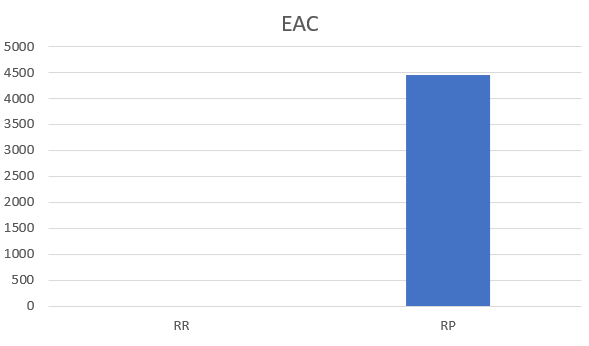
\includegraphics[scale=0.8]{src/ResocontoVerifica/src/img/EAC.png}
	\caption{Estimated At Completion durante i periodi da RR a RP}
\end{figure}


\subsubsection{VAC - Variance At Completion}
\rowcolors{2}{\evenRowColor}{\oddRowColor}
\renewcommand{\arraystretch}{1.5}
\begin{longtable}{ C{3cm} C{3cm}  C{3cm}  C{3cm} c }
    \caption{ VAC nei periodi da RR a RP} \\
    \rowcolor{\primaryColor}
    \textcolor{\secondaryColor}{
    \centering\textbf{RR}}     & \textcolor{\secondaryColor}{\centering\textbf{RP}}    & \textcolor{\secondaryColor}
    {\centering\textbf{RQ}} & \textcolor{\secondaryColor}{\centering\textbf{RA}}    \\
    \textit{-}           & 2,86\%                                 & - & - \\
\end{longtable}


\begin{figure}[H]
	\centering
	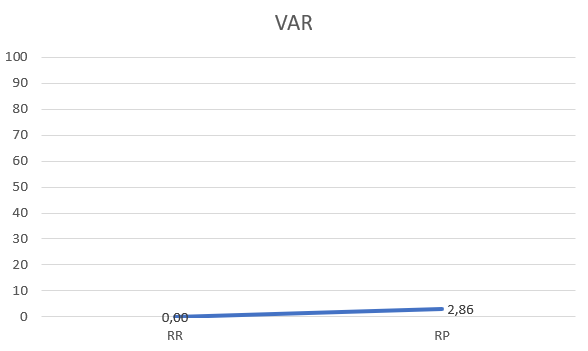
\includegraphics[scale=0.8]{src/ResocontoVerifica/src/img/VAC.png}
	\caption{Variance At Completion durante i periodi da RR a RP}
\end{figure}

\subsubsection{AC - Actual Cost}
\rowcolors{2}{\evenRowColor}{\oddRowColor}
\renewcommand{\arraystretch}{1.5}
\begin{longtable}{ C{3cm} C{3cm}  C{3cm}  C{3cm} c }
    \caption{ AC nei periodi da RR a RP} \\
    \rowcolor{\primaryColor}
    \textcolor{\secondaryColor}{
    \centering\textbf{RR}}     & \textcolor{\secondaryColor}{\centering\textbf{RP}}    & \textcolor{\secondaryColor}
    {\centering\textbf{RQ}} & \textcolor{\secondaryColor}{\centering\textbf{RA}}    \\
    \textit{-}           & 4463,00\euro                                  & - & - \\
\end{longtable}

\begin{figure}[H]
	\centering
	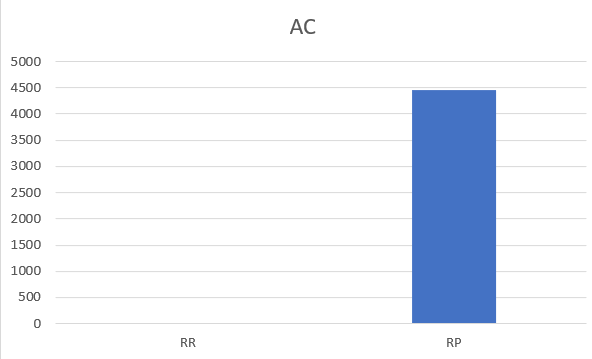
\includegraphics[scale=0.8]{src/ResocontoVerifica/src/img/AC.png}
	\caption{ Actual Cost durante i periodi da RR a RP}
\end{figure}


\subsubsection{Indice di Gulpease}
Nella seguente tabella vengono riportati gli indici Gulpease\glo{} di tutti
i documenti prodotti finora.
    \rowcolors{2}{\evenRowColor}{\oddRowColor}
\renewcommand{\arraystretch}{1.5}
\begin{longtable}{ c c  C{4cm}  c  c }
    \caption{Tabella dell'indice di Gulpease RR} \\
    \rowcolor{\primaryColor}
    \textcolor{\secondaryColor}{
    \centering\textbf{Documento}}     & \textcolor{\secondaryColor}{\centering\textbf{Indice Gulpease}}    & \textcolor{\secondaryColor}
    {\centering\textbf{Esito}} \\
    \textit{Analisi dei Requisiti v1.0.0}           & 62                                    & Superato{} \\
    \textit{Glossario v1.0.0}                       & 72                                    & Superato{} \\
    \textit{Norme di Progetto v1.0.0}               & 68                                   & Superato{} \\
    \textit{Piano di Progetto v1.0.0}                & 64                                    & Superato{} \\
    \textit{Piano di Qualifica v1.0.0}                & 59                                    & Superato{} \\
    \textit{Studio di Fattibilità v1.0.0}               & 69                                    & Superato{} \\
    \textit{Verbale Interno 2020-10-31 v1.0.0}          & 72                                    & Superato{} \\
    \textit{Verbale Interno 2020-11-12 v1.0.0}          & 69                                    & Superato{} \\
    \textit{Verbale Interno 2020-12-11 v1.0.0}          & 73                                    & Superato{} \\
    \textit{Verbale Esterno 2020-12-18 v1.0.0}          & 76                                    & Superato{} \\
    \textit{Verbale Interno 2020-12-22 v1.0.0}          & 71                                    & Superato{} \\
    \textit{Verbale Interno 2021-01-05 v1.0.0}          & 74                                    & Superato{} \\
    \textit{Verbale Interno 2021-01-10 v1.0.0}          & 70                                    & Superato{} \\

\end{longtable}

\rowcolors{2}{\evenRowColor}{\oddRowColor}
\renewcommand{\arraystretch}{1.5}
\begin{longtable}{ c c  C{4cm}  c  c }
    \caption{Tabella dell'indice di Gulpease RP} \\
    \rowcolor{\primaryColor}
    \textcolor{\secondaryColor}{
    \centering\textbf{Documento}}     & \textcolor{\secondaryColor}{\centering\textbf{Indice Gulpease}}    & \textcolor{\secondaryColor}
    {\centering\textbf{Esito}} \\
    \textit{Analisi dei Requisiti v2.0.0}           & 70                                    & Superato{} \\
    \textit{Glossario v2.0.0}                       & 73                                    & Superato{} \\
    \textit{Norme di Progetto v2.0.0}               & 72                                   & Superato{} \\
    \textit{Piano di Progetto v2.0.0}                & 65                                    & Superato{} \\
    \textit{Piano di Qualifica v2.0.0}                & 68                                    & Superato{} \\
    \textit{Verbale Esterno 2021-01-22 v1.0.0}          & 71                                    & Superato{} \\
    \textit{Verbale Interno 2020-01-29 v1.0.0}          & 69                                    & Superato{} \\
    \textit{Verbale Interno 2020-02-10 v1.0.0}          & 73                                    & Superato{} \\
    \textit{Verbale Esterno 2020-02-18 v1.0.0}          & 68                                    & Superato{} \\
    \textit{Verbale Interno 2020-02-25 v1.0.0}          & 70                                    & Superato{} \\
    \textit{Verbale Interno 2020-03-06 v1.0.0}          & 67                                    & Superato{} \\
\end{longtable}

\begin{figure}[H]
	\centering
	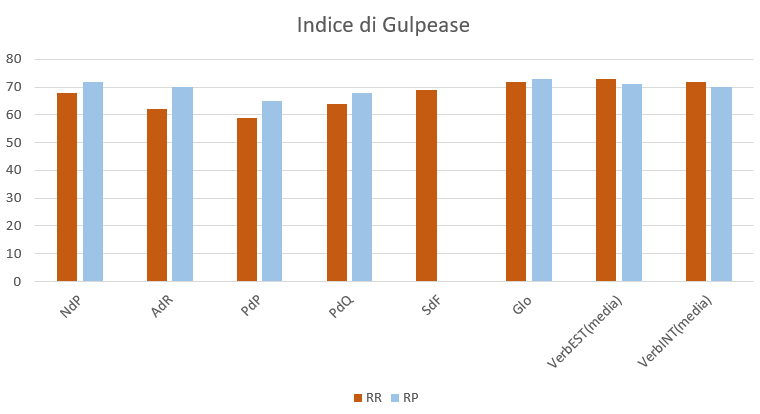
\includegraphics[scale=0.8]{src/ResocontoVerifica/src/img/indiceGulpease.png}
	\caption{Indice di Gulpease}
\end{figure}



